\chapter{Análise de Requisitos}

\section{Modelo Conceitual}

% \begin{figure}[!h]
%  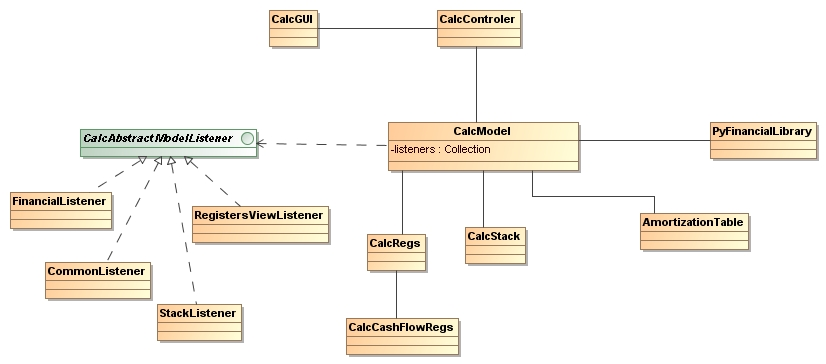
\includegraphics[height = 8cm]{CalcDC.jpg}
%  \caption{\it Modelo Conceitual da PyFinancial.} \label{fig:modConc}
% \end{figure}

\begin{figure}[!h]
 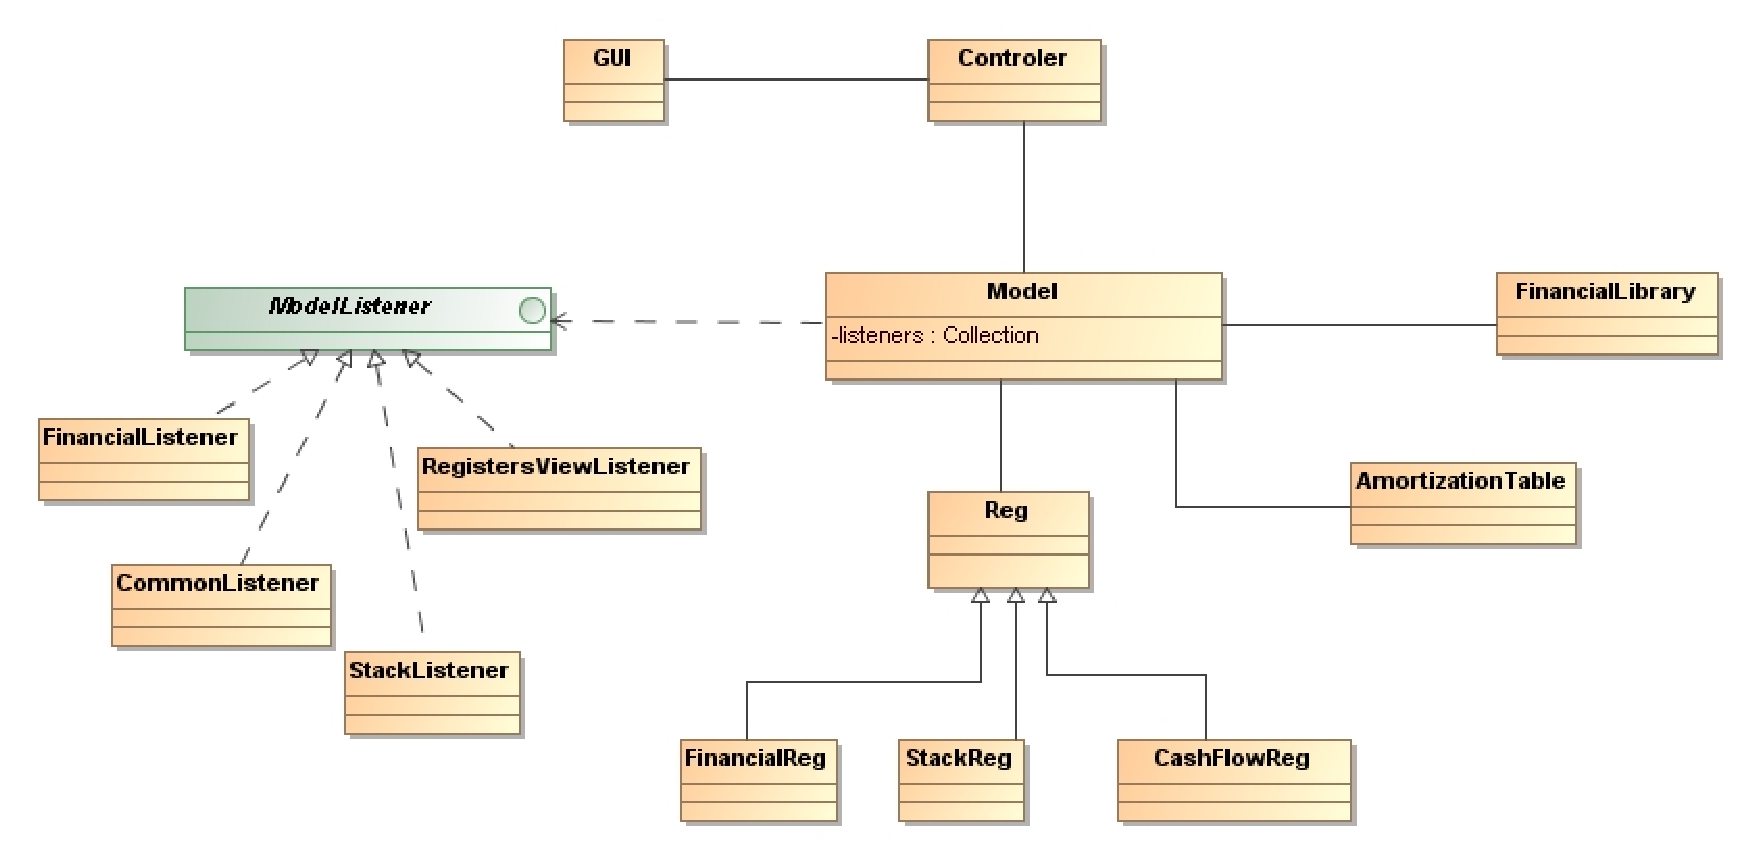
\includegraphics[scale=0.5]{CalcDC.eps}
 \caption{\it Tabela que descreve quando as atividades de XP1 devem ser realizadas.} \label{tab:modeConc}
\end{figure}

A figura \ref{tab:modeConc} apresenta o modelo conceitual da calculadora financeira, objetivo central desse projeto. É possível identificar algumas entidades centrais desse sistema são elas:

\begin{itemize}
	\item Model
	\item GUI
	\item Controler
	\item AbstractModelListener
	\item Reg
	\item FinancialLibrary
\end{itemize}

\subsection{Model}
Módulo central da aplicação que será responsável por fazer a troca de mensagens entre as demais entidades do sistema as quais está conectada, bem como realizar toda a manipulação de registradores (pilha, financeiros e demais registradores comuns) e funções de modo a efetivar as funcionalidades requisitadas pelo usuário. Também é de sua responsabilidade receber e preparar os dados da aplicação para posterior manipulação, dados esses captados pela interface. Por fim, esta entidade também é responsável por persistir os registradores quando necessário, bem como todo o estado interno da calculadora previamente configurada pelo usuário.

\subsection{GUI}
Esta é a entidade que estará em contato direto com o usuário da aplicação. Logo, este é o módulo que receberá os dados externos e os transmitirá para entidades mais internas, assim como receberá os resultados das operações realizadas pela calculadora e os transmitirá ao cliente de uma maneira mais amigável. Essa interface também é responsável por apresentar os dados segundo preferências do usuário previamente selecionadas, por exemplo, com um dado número de casas decimais.

\subsection{Controller}
Esta entidade é o controlador do sistema, responsável por desacoplar a interface da camada de negócios do sistema. Receberá as requisições feitas pelo cliente da aplicação, através da interface (\textit{GUI}), e identificará as operações correspondentes no \textit{Model} que se responsabilizarão por realizar as atividades correspondentes.

\subsection{AbstractModelListener}
Entidade abstrata da qual outras a generalizarão. Estas serão responsáveis por capturar qualquer mudança importante ocorrida no \textit{Model} que seja de interesse do usuário. Assim essas alterações serão refletidas na interface. Aqui encaixa-se situações como requisições de realização de operações matemáticas/financeiras, manipulações de registradores, etc.

\subsection{Reg}
Entidade que representa o papel de um registrador. Um registrador é um importante elemento usado para a realização das atividades objetivo da calculadora. Neles armazena-se os valores a serem utilizados nas operações, bem como os resultados das operações requisitadas. Esta entidade será especializada por outras adicionando as particularidades pertinentes aos diferentes tipos de registradores.

\subsection{FinancialLibrary}
Entidade que representa a biblioteca das funções financeiras. Todo e qualquer cálculo financeiro deve chamar a operação correspondente na biblioteca garantindo uma melhor organização e consequentemente, a separação de interesses.

Essa é a entidade que poderá vir a ser utilizada por programadores Python, incluindo os membros da equipe, para desenvolvimento das mais variadas aplicações que necessitem da realização de funções financeiras.

\section{Requisitos}

Durante as reuniões de planejamento entre os membros da equipe, o cliente e possíveis usuários dos nossos produtos, um conjunto de requisitos funcionais e não funcionais ficaram estabelecidos. São eles:

\begin{itemize}
 \item \textbf{Requisitos Funcionais}
	\begin{itemize}
 	\item O usuário deverá ser capaz de realizar as operações matemáticas/financeiras seguindo a Notação Polonesa Reversa \cite{NPR}.
	\item O usuário deve ser capaz de especificar o número de casas decimais apresentadas, bem como requisitar a apresentação dos valores em notação científica.
	\item O usuário deve ser capaz de adicionar/limpar valores em todos os 30 registradores existentes na calculadora. 
	\item O usuário deve ser capaz de realizar operações matemáticas básicas: soma ($+$),subtração ($-$), divisão ($/$) e multiplicação ($*$). Deve também ser capaz de realizar operações mais avançadas: exponenciação ($ e^{x} $), quadrado de um número ($x^{2}$), logaritmo natural ($\ln$), potência de números ($y^{x}$), raiz quadrada ($x^{1/2}$), percentual do total ($\%T$), variação percentual ($\Delta\%$) e percentual de um número ($\%$).
	\item O usuário deverá ser capaz de realizar cálculos que descubram os principais valores financeiros: número de períodos (n), taxa de juros (i), valor present (PV), valor da parcela (PMT) e valor futuro (FV). Esses cálculos podem envolver ou não multiplos fluxos de caixa.
	\item O usuário deve ser capaz de realizar análises de investimentos mais apuradas através do cálculo do valor presente líquido (NPV), bem como da taxa interna de retorno (IRR).
	\item O usuário deve ser capaz de calcular a amortização de suas dívidas no sistema de amortização francês (SAF), bem como no sistema de amortização constante (SAC). Apresentando uma tabela de amortização ao final.
	\item O usuário deve ser capaz de realizar a conversão entre taxas de juros anuais para taxas de juros mensais tanto no sistema de juros simples, como no sistema de juros compostos. Além disso, deve ser capaz de converter um número de períodos anuais em períodos mensais.
	\item O usuário deve ser capaz de rotacionar os valores dos registradores da pilha de cima para baixo.
	\item Ao finalizar o uso os dados da tela e dos registradores devem ser armazenados em algum tipo de persistência.
	
	\end{itemize}
 \item \textbf{Requisitos Não-Funcionais}
	\begin{itemize}
	 \item \textbf{Interface}. Possuir interface similar a da calculadora HP12-C, com melhoramentos que possam facilitar sua utilização.
	 \item \textbf{Usabilidade}. O nível de dificuldade encontrado para uso de nossa calculadora deve ser o mesmo encontrado quando faz-se uso das calculadoras tradicionais.
	 \item \textbf{Volume de Utilização}. A calculadora será mono-usuário, porém devendo ser robusta o suficiente para ser utilizada durante um longo intervalo de tempo ininterruptamente sem apresentar problemas.
	 \item \textbf{Hardware e software alvo}. A calculadora deverá funcionar no Internet Tablet N800 da Nokia, no sistema operacional Maemo Diablo (4.1.x) 
	 \item \textbf{Qualidade}. Com relação a precisão, deseja-se que os valores calculados em nossa calculadora não devam diferir em mais de $0.001$ unidades dos valores calculados na HP12-C original.
	 \item \textbf{Expressividade nas mensagens}. Entradas equivocadas do usuário deverão apresentar mensagens de erros que sejam mais intuitivas do que as apresentadas pela calculadora original (e.g. "Erro 6").
	 \item \textbf{Desempenho}. O tempo de resposta dos resultados não deve ultrapassar o tempo que a calculadora HP12-C leva para executar as mesmas operações (considerando que só o programa da calculadora esteja em execução).
	 \item \textbf{Segurança}. Os arquivos que conterão os valores dos registradores recém utilizados pelo usuário deverão ficar protegidos de alteração externa.
	 \item \textbf{Compatibilidade}. É desejável que a aplicação possa ser portada para versões mais novas do dispositivo alvo, como o N810, bem como para novas versões do Maemo.
	 \item \textbf{Internacionalização}. A calculadora deve ser desenvolvida para tornar possível a internacionalização. 
	 \item \textbf{Packaging}. A distribuição do aplicativo deve ser realizada através de um arquivo .deb que servirá como instalador para o mesmo.
	\end{itemize}
\end{itemize}
